%:Clase del documento
\documentclass[fontsize=10pt, Myfinal=true, twoside, numbers=noenddot]{scrbook}
%Minion=true, English=true, Myfinal=true

%:Paquete de estilos propuesto
\usepackage{libroETSI}

%:Paquete específico para cargar tikz (y sus librerías) y pgfplots
\usepackage{dtsc-creafig}

%:Paquete para notaciones específicas
\usepackage{notacion}

%:Paquete para incorporar aspectos concretos de la edición
\usepackage{edicionPFC}


%:Estas líneas de código son INNECESARIAS excepto para mostrar determinadas características en este manual. Pueden eliminarse o comentarse sin ningún problema.
%Se usan para compilar el capítulo estilolibroetsi.tex
\usepackage[final]{showexpl}
\lstset{explpreset={frame=none,rframe={}, numbers=none,numbersep=3pt, columns=flexible,language={[LaTeX]TeX},basicstyle=\ttfamily,keywordstyle=\color{blue}}}%numberstyle=\tiny,

%:Para modificar fácilmente la fuente del texto.
\makeatletter
\ifdtsc@Minion % Queremos utilizar la fuente Minion y lo hemos declarado al principio
	\ifluatex
		\setmainfont[Renderer=Basic, Ligatures=TeX,	% Fuente del texto 
		Scale=1.01,
		]{Minion Pro}
   		% En este caso conviene modificar ligeramente el tamaño de las fuentes matemáticas
		\DeclareMathSizes{10}{10.5}{7.35}{5.25}
		\DeclareMathSizes{10.95}{11.55}{8.08}{5.77}
		\DeclareMathSizes{12}{12.6}{8.82}{6.3}
%		\setmainfont[Renderer=Basic, Ligatures=TeX,	% Fuente del texto 
%		]{Adobe Garamond Pro}
%		\setmainfont[Renderer=Basic, Ligatures=TeX,	% Fuente del texto 
%		]{Palatino LT Std}
	\fi
\else
	\ifluatex
		% Para utilizar la fuente Times New Roman, o alguna otra que se tenga instalada
		\setmainfont[Renderer=Basic, Ligatures=TeX,	% Fuente del texto 
		Scale=1.0,
		]{Times New Roman}
	\else
		\usepackage{tgtermes} 	%clone of Times
		%\usepackage[default]{droidserif}
		%\usepackage{anttor} 	
	\fi
\fi
\makeatother

%Por si quieren usar bibliografía con BIBER
%BIBER%%:Para la bibliografía en BIBER, descomentar las líneas siguientes
%\defbibheading{etsi}[]{%
%	\chapter*{Bibliografía}%
%	\chaptermark{Bibliografía} 
%	\markboth{#1}{#1}}
%\addbibresource{bibliografiaLibroETSI.bib}

% Ejemplo de Glosario
\newacronym[type=main]{ETSI}{ETSI}{Escuela Técnica Superior de Ingeniería}
\newacronym[type=main]{US}{US}{Universidad de Sevilla}
\newacronym[type=main]{DMC}{DMC}{Canal Discreto sin Memoria}


\makeindex
\makeglossaries %Si no se quiere el glosario, comentar esta línea.

% Formato A4
\geometry
{paperheight=297mm,%
paperwidth=210mm,%
top=25mm,%
headsep=8.5mm,%
includefoot, 
textheight=240mm, 
textwidth=150mm, 
bindingoffset=0mm, 
twoside}

\usepackage[a4,center]{crop}%para poner las cruces de esquina de página, poner la opción cross

%:Esquema de numeración por defecto
\setenumerate[1]{label=\normalfont\bfseries{\arabic*.}, leftmargin=*, labelindent=\parindent}
\setenumerate[2]{label=\normalfont\bfseries{\alph*}, leftmargin=*}
\setenumerate[3]{label=\normalfont\bfseries{\roman*.}, leftmargin=*}
\setlist{itemsep=.1em}
\setlength{\parindent}{1.0 em}

\setcounter{tocdepth}{4}						% El nivel hasta el que se muestra el índice 


%:Empieza el documento

\begin{document}
%:Para incluir toda la referencia bibliográfica aunque no se cite, descomente la siguiente línea
%\nocite{*}


%PORTADA
%ver edicionPFC.sty para modificaciones

%:Para crear la portada y la portada interior (pagina titular)
\titulo{Entrenamiento y despliegue de un modelo \\ de clasificación de audio} %\mbox evita que se divida una palabra al cambiar de línea
\autor{Antonio José Aragón Molina}
\director{María del Mar Elena Pérez}
\titulodirector{Profesor Titular}

\departamento{Dpto. Ingeniería Electrónica}
\centro{Escuela Técnica Superior de Ingeniería}
\universidad{Universidad de Sevilla}
\titulacion{Máster en Ingeniería de Telecomunicación}
% current year
\fecha{\today} %Fecha de defensa, mes y año
\nombretrabajo{Trabajo Fin de Máster} %Trabajo Fin de Grado, Proyecto fin de Máster,....

\hypersetup
{
linkcolor=black, %Tocar para poner color en enlaces
pdfauthor={\elautor},
pdftitle={\nombretrabajo,\eltitulo}, 
pdfkeywords={Latex, edición, formato de texto}	
}

\portadaPFC{figuras/LogoUS.pdf}{figuras/LogoTSC.pdf} %logo de la Universidad y logo del departamento, si lo hubiera. Para cambiar el pie de página con los logos, debe editarse el fichero ediciónPFC.sty

%Fin Portada

%:Todo lo que constituye la primera parte del libro que no es el cuerpo del libro en realidad
\frontmatter
\pagenumbering{Roman} %Pone la numeración en mayúscula (En español parece que es obligatorio)

%\include{dedicatoria/dedicatoria}%¿Comentar para proyectos/tesis?
% !TEX root =../LibroTipoETSI.tex
\chapter*{Agradecimientos}
%\pagestyle{especial}
\pagestyle{empty}
%\chaptermark{Agradecimientos}
\phantomsection
%\addcontentsline{toc}{listasf}{Agradecimientos}
%\vspace{1cm}
%{\huge{Agradecimientos}}
%\vspace{1cm}

\lettrine[lraise=-0.1, lines=2, loversize=0.25]{A} mis padres, por su apoyo incondicional, por su paciencia y por su amor.
A mis profesores y profesoras, por su dedicación y su esfuerzo.
A mis compañeros de clase, por acompañarme en este camino.
A mis compañeros de piso, por su compañía y su apoyo.
A mis amigos de siempre, gracias por sacarme siempre una sonrisa.
A la música, por hacerme sentir.



%gradecemos}, a todos nuestros maestros, cuanto nos enseñaron.

{\flushleft{\hfill \emph{Antonio José Aragón Molina}}}%
\vspace{-.3cm}
{\flushleft{\hfill \emph{Escuela Técnica Superior de Ingeniería}}}%
{\flushleft{\hfill \emph{Sevilla, \today}}}%

%PFC/PFM/TESIS
% !TEX root =../LibroTipoETSI.tex
\chapter*{Resumen}
\pagestyle{especial}
\chaptermark{Resumen}
\phantomsection
\addcontentsline{toc}{listasf}{Resumen}

\lettrine[lraise=-0.1, lines=2, loversize=0.2]{E}{n} nuestra Escuela se producen un número considerable de documentos, tantos docentes como investigadores. Nuestros alumnos también contribuyen a esta producción a través de sus trabajos de fin de grado, máster y tesis. El objetivo de este material es facilitar la edición de todos estos documentos y a la vez fomentar nuestra imagen corporativa, facilitando la visibilidad y el reconocimiento de nuestro Centro.

%La hoja de estilo utilizada es una versión de la que el Prof. Payán realizó para un libro que desde hace tiempo viene escribiendo para su asignatura. Con ella se han realizado estas notas, a modo de instrucciones, añadiéndole el diseño de la portada. El diseño de la portada está basado en el que el prof. Fernando García García, de nuestra universidad, hiciera para los libros de la sección de publicación de nuestra Escuela.


\chapter*{Abstract}
\pagestyle{especial}
\chaptermark{Abstract}
\phantomsection
\addcontentsline{toc}{listasf}{Abstract}

\lettrine[lraise=-0.1, lines=2, loversize=0.2]{I}{n} our school there are a considerable number of documents, many teachers and researchers. Our students also contribute to this production through its work in order of degree, master's theses. The aim of this material is easier to edit these documents at the same time promote our corporate image, providing visibility and recognition of our Center. 

...
\emph{-translation by google-}

 

% Índice abreviado 
% El índice abreviado se incluye también en algunos libros, con menor detalle que el completo. Descomentar las siguientes líneas.
\cleardoublepage
\phantomsection
\addcontentsline{toc}{listasf}{Índice Abreviado}
\pagestyle{especial}
\shorttoc{Índice Abreviado}{1}

%Índice normal, el completo
\cleardoublepage
\phantomsection
\pagestyle{especial}
\tableofcontents


% %:---------------------------Notación 
%Toda esta notación es opcional, pero creemos que puede ser de mucha ayuda.
%Juan José Murillo Fuentes y Javier Payán Somet. Copyright 2011. Todos los derechos reservados.

%:---------------------------------------------------  Referencias
%Puede usar los comandos \label y \ref, pero con lo de abajo se facilita el uso de múltiples etiquetas para ecuaciones, secciones,...
%Etiquetas:
\newcommand{\LABEQ}[1]{\label{eq:#1}}%\mathtt{[eq:#1]}\qquad %Equación
\newcommand{\LABALG}[1]{\label{alg:#1}}%\mathtt{[lab:#1]}\qquad %Algoritmo
\newcommand{\LABTAB}[1]{\label{tab:#1}}%{\tt [tab:$\text{$#1$}$]}} %Tabla
\newcommand{\LABFIG}[1]{\label{fig:#1}}%{\tt [fig:$\text{$#1$}$]}} %Figura
\newcommand{\LABTHM}[1]{\label{thm:#1}}%{\tt [thm:#1]}} % Teorema
\newcommand{\LABPRP}[1]{\label{prp:#1}}%{\tt [prp:#1]}} % Proposición
\newcommand{\LABLEM}[1]{\label{lem:#1}}%{\tt [lem:#1]}} % Lema
\newcommand{\LABCOR}[1]{\label{cor:#1}}%{\tt [cor:#1]}} %Corolario 
\newcommand{\LABDFN}[1]{\label{dfn:#1}}%{\tt [dfn:#1]}} %Definición
%\newcommand{\LABFNT}[1]{\label{fnt:#1}}%{\tt [fnt:#1]}} %
%
%Referencias a las etiquetas anteriores, Incluyen el título. Puede cambiarlos aquí. Por ejemplo, si quiere "Fig." en vez de "Figura"...
\newcommand{\EQ}[1]{\eqref{eq:#1}}%$^{\text{\tt [#1]}}$} %used to be {(\ref{eq:#1})}
\newcommand{\ALG}[1]{~\ref{alg:#1}}
%\newcommand{\TAB}[1]{Tabla ~\ref{tab:#1}}%$^{\text{\tt [#1]}}$}
\newcommand{\TAB}[1]{\autoref{tab:#1}}%$^{\text{\tt [#1]}}$}
%\newcommand{\FIG}[1]{Figura~\ref{fig:#1}} %$^{\text{\tt [#1]}}$} 
\newcommand{\FIG}[1]{\autoref{fig:#1}} %$^{\text{\tt [#1]}}$} 

%\newcommand{\FIG}[1]{Fig. \ref{fig:#1}} %$^{\text{\tt [#1]}}$} 
\newcommand{\THM}[1]{Teorema~\ref{thm:#1}}%$^{\text{\tt [#1]}}$}
\newcommand{\COR}[1]{Corolario~\ref{cor:#1}}%$^{\text{\tt [#1]}}$}
\newcommand{\PRP}[1]{Propiedad~\ref{prp:#1}}%$^{\text{\tt [#1]}}$}
\newcommand{\LEM}[1]{Lema~\ref{lem:#1}}%$^{\text{\tt [#1]}}$}
\newcommand{\DFN}[1]{Definición~\ref{dfn:#1}}%$^{\text{\tt [#1]}}$}
%\newcommand{\FNT}[1]{~\ref{fnt:#1}}%$^{\text{\tt [#1]}}$}

%Etiquetas para títulos tipo capítulo, sección, subsección,...
\newcommand{\LABCHAP}[1]{\label{chap:#1}}%{\tt [chap:#1]}}
\newcommand{\LABAPEN}[1]{\label{apen:#1}}%{\tt [chap:#1]}}
\newcommand{\LABSEC}[1]{\label{sec:#1}}%{\tt [sec:#1]}}
\newcommand{\LABSSEC}[1]{\label{ssec:#1}}%{\tt [ssec:#1]}}
\newcommand{\LABSSSEC}[1]{\label{sssec:#1}}%{\tt [sssec:#1]}}
%
%Referencias para los anteriores títulos
\newcommand{\CHAP}[1]{Capítulo~\ref{chap:#1}}%$^{\text{\tt [c:#1]}}$}
\newcommand{\SEC}[1]{Sección~\ref{sec:#1}}%$^{\text{\tt [s:#1]}}$}
\newcommand{\SSEC}[1]{Subsección~\ref{ssec:#1}}%$^{\text{\tt [ss:#1]}}$}
\newcommand{\SSSEC}[1]{Apartado~\ref{sssec:#1}}%$^{\text{\tt [sss:#1]}}$}
\newcommand{\APEN}[1]{Apéndice~\ref{apen:#1}}%$^{\text{\tt [c:#1]}}$}
%
%%
%\newcommand{\PAGEEQ}[1]{~\pageref{eq:#1}}
%\newcommand{\PAGETAB}[1]{~\pageref{tab:#1}}
%\newcommand{\PAGEFIG}[1]{~\pageref{fig:#1}}


%%%%Definiendo caligrafías especiales 
%\newcommand{\emphb}[1]{\emph{\textbf{#1}}}
%\newcommand{\X}{\calg{X}} %{\ensuremath{\calg{X}}} %\textrm{\ifmmode {1pt} \else {\, } \fi}
%\newcommand{\Y}{\calg{Y}}%{\ensuremath{\calg{Y}}}
\newcommand{\calg}[1]{\ensuremath{\mathcal{#1}}} %JJMF: No entiendo para qué es esto.
%\newcommand{\hb}[1]{\ensuremath{\textrm{\usefont{T1}{phv}{b}{n}#1}}}
%\newcommand{\hn}[1]{\ensuremath{\textrm{\usefont{T1}{phv}{m}{n}#1}}}

%
%:Renombrando overline
%\newcommand{\overl}[1]{\bar{#1}}

\DeclarePairedDelimiter\ceil{\lceil}{\rceil}
\DeclarePairedDelimiter\floor{\lfloor}{\rfloor}

%%%% vectores
%
\newcommand{\vect}[1]{\mathbf{#1}}     %vectors (bold type)
\newcommand{\vc}[1]{\mathbf{#1}}     %vectors (bold type)
\newcommand{\matr}[1]{\mathbf{#1}}     %matrices (bold type)
% ó:
%\newcommand{\vc}[1]{\ensuremath{\mathbf{#1}}}
% ó:
%\newcommand{\vct}[1]{\boldsymbol{#1}}
%\newcommand{\vect}[1]{\boldsymbol{#1}}  %vectors (bold type)
%\newcommand{\matr}[1]{\boldsymbol{#1}}  %matrices (bold type)

\renewcommand*{\j}{\ensuremath{\textrm{j}}}%{\mathop{}\mathrm{j}}

%%%% Complejos y exponenciales
\newcommand{\xp}[1]{\e^{\j{#1}}}         %simple exponential
\newcommand{\xppi}[1]{\e^{\j2\pi{#1}}}         %simple exponential
\newcommand{\nxp}[1]{\e^{-\j{#1}}}       %negative exponential
\newcommand{\nxppi}[1]{\e^{-\j2\pi{#1}}}       %negative exponential
\newcommand{\e}{\mathrm{e}}
%\newcommand{\xp}[1]{\e^{j{#1}}}         %simple exponential
%\newcommand{\nxp}[1]{\e^{-j{#1}}}       %negative exponential
%
%
% Parte real
\newcommand{\re}{\mbox{$\mathrm{I\!Re}$}}       %real part
%\renewcommand{\Re}{\ensuremath{\boldsymbol{\mathcal{R}}}}
%\renewcommand{\Re}{\ensuremath{\textrm{\usefont{T1}{phv}{m}{n}Re}}}
% Parte imaginaria
\newcommand{\im}{\mbox{$\mathrm{I\!Im}$}}       %imaginary part
%\renewcommand{\Im}{\ensuremath{\boldsymbol{\mathcal{I}}}}
%\renewcommand{\Im}{\ensuremath{\textrm{\usefont{T1}{phv}{m}{n}Im}}}
%:Creando la unidad imaginaria
%\renewcommand{\j}{\ensuremath{\textrm{\usefont{T1}{lmr}{m}{n}j}}}


%%%% Maths functions and symbols
%
%:Para definir funciones matemáticas en castellano
\makeatletter
\ifdtsc@English
	\DeclareMathOperator{\sen}{sin}
	\DeclareMathOperator{\tg}{tg}  %tg() function
	\DeclareMathOperator{\arctg}{arctg}     %arctg() function
\fi
\makeatother

\DeclareMathOperator{\sa}{Sa}
%
\DeclareMathOperator{\sgn}{sgn}
%\newcommand{\sgn}{\mathrm{sign}}        %sign() function
%\newcommand{\sign}{\mathrm{sign}}
%
\DeclareMathOperator{\rect}{rect}
\DeclareMathOperator{\sinc}{Sinc}
%\newcommand{\cost}{\psi}                %cost or contrast function
\newcommand{\pder}[2]{\frac{\partial #1}{\partial #2}}  %partial derivative
%
%
%\renewcommand{\mod}{\bmod}      %\:\text{mod}\:}
\newcommand{\RR}{\mathbb{R}}            %real numbers
\newcommand{\CC}{\mathbb{C}}    %complex numbers
%
%\newcommand{\tg}{\mahtrm{tg}}           
%\newcommand{\angl}{\arg}
%
\newcommand{\costo}[2]{\cos^{#1}\!#2}   %cos to power
\newcommand{\sento}[2]{\sin^{#1}\!#2}   %sen to power
%
\newcommand{\gra}{\ensuremath{^\circ}}  %Grados. Ejemplo: $5\gra$ K serían 5º K


%%%% Matrices, traspuesta, hermítica, ...
%
\newcommand{\inv}{^{-1}}                %inverse operator
\newcommand{\trs}{^\top}                %transposition operator
%\newcommand{\trs}{^{\textrm{\usefont{T1}{phv}{b}{n}{T}}}}          %transponer una matriz
\newcommand{\psd}{^\dagger}             %pseudoinverse operator
\newcommand{\cnj}{^*}                   %complex conjugate
\newcommand{\pcnj}{^{\phantom{*}}}      %phantom complex conjugate (for alignment)
\newcommand{\her}{^\mathrm{H}}          %complex conjugate transpose
%\newcommand{\her}{^{\textrm{\usefont{T1}{phv}{b}{n}{H}}}}          %Hermítica
\newcommand{\id}[1]{\vect{I}_{#1}}       %identity matrix
%\newcommand{\id}{\matr{I}}       %identity matrix
\newcommand{\diag}[1]{\mathrm{diag}\left(#1\right)}     %diagonal
%\DeclareMathOperator{\diag}{diag}



%%%% indices de prestaciones %%%%%%%%%
%
%\newcommand{\isr}{\mathrm{ISR}}           %interference-to-signal ratio
\newcommand{\snr}{\mathrm{SNR}}           %signal-to-noise ratio
\newcommand{\mse}{\mathrm{MSE}}           %minimum mean square error
%
%ó se pueden escribir como
%\newcommand{\SNR}{\ensuremath{\textrm{SNR}}}
%...


%%%%Miscellaneos
%
%Redefiniendo epsilon
%\renewcommand{\epsilon}{\ensuremath{\textrm{\usefont{OML}{cmr}{m}{n}\symbol{15}}}}
%
%:Creando ``tal que'' de las expresiones matemáticas
\newcommand{\talq}{\colon}
%
%%Creando ``igual por definición'' de las expresiones matemáticas
\newcommand{\eqdef}{\ensuremath{\mathrel{\stackrel{\mathrm{def}}{=}}}}
%%ó
%\newcommand{\eqdef}{\triangleq}         %equal by definition
%
%
%:Creando la igualdad basada en una ecuación
%\newcommand{\igualref}[1]{\ensuremath{\mathrel{\stackrel{\mathrm{\eqref {#1}}}{=}}}}
%
%:Definiendo cardinal y norma
\newcommand{\norm}[1]{\ensuremath{\left\lVert #1 \right\rVert }}
\newcommand{\card}[1]{\ensuremath{\left| #1\right|}}
%\newcommand{\card}[1]{\ensuremath{\text{card}~#1}
%
%:Renombrando \boldsymbol
%\newcommand{\bm}[1]{\boldsymbol{#1}}
%
%:Facilitando la escritura de X_{i}
\newcommand{\xyz}[3]{\ensuremath{#1_{#2},#2=1,2,\ldots,#3}}
%
%:Creando el diferencial. Por defecto, dx
%\newcommand*{\df}[1][x]{\mathop{}\!\mathrm{d}{#1}}
\newcommand{\df}[1]{\mathrm{d}{#1}}

%
%%Modificando el menor igual y el mayor igual
\renewcommand{\le}{\leqslant}           %fancy \le
\renewcommand{\ge}{\geqslant}           %fancy \ge
%
%:Creando BL=backslash de las expresiones matemáticas
\newcommand{\BL}{\ensuremath{\backslash}}
%
%Redefiniendo iff
\renewcommand{\iff}{\Leftrightarrow}
%
%\newcommand{\what}{\widehat}
%\newcommand{\supp}[1]{^{(#1)}}          %superindex with parentheses
\newcommand{\eqexpl}[1]{\underset{#1}{\underset{\uparrow}{=}}}  %equal with explanation
%\newcommand{\proof}{\noindent {\bf Proof.} }
%\newcommand{\skproof}{\noindent {\bf Sketch of the proof.} }
\newcommand{\sfrac}[2]{\tfrac{#1}{#2}}  %small frac
\newcommand{\inc}{\Delta}
\newcommand{\ten}[1]{\cdot 10^{#1}}     %scientific notation
%\newcommand{\arrow}{$\rightarrow$ }
%\newcommand{\darrow}{$\Rightarrow$ }
%\newcommand{\tends}{\rightarrow}                         %'tends to'
\newcommand{\tendsub}[1]{\xrightarrow[#1]{}}             %{\underset{#1}{\longrightarrow}} %'tends to' with subscript
%\newcommand{\tendsubsup}[2]{\xrightarrow[#1]{#2}}        %{\overset{#2}{\tendsub{#1}}}   %'tends to' with sub and superscript
\newcommand{\ord}{\mathrm{O}}         %order of magnitude
\newcommand{\tm}{^{\text{\tiny{TM}}}} %trademark
%
%
%:Creando ``L'' de las expresiones matemáticas
%\renewcommand{\L}[1][L\!]{\ensuremath{\boldsymbol{\mathcal{#1}}}}
%\renewcommand{\L}[1][L\!]{\ensuremath{\boldsymbol{\mathscr{#1}}}}
%
%:Creando la F de transformada de Fourier
%\newcommand{\Fo}{\ensuremath{\boldsymbol{\mathscr{F}}}}
%
%:Creando la H de transformada de Hilbert
%\newcommand{\Hi}{\ensuremath{\boldsymbol{\mathscr{H}}}}
%
%
%%%% Indention
%
%\newcommand{\ind}{$\phantom{\indent}$}
%


%%%% Basic statistics
%
%%Creando el operador "valor esperado" 
%\newcommand{\E}{\ensuremath{\mathbb{E}}}
%\newcommand{\E}{\ensuremath{\textrm{\usefont{OML}{phv}{b}{n}E\hspace{1pt}}}}
%\newcommand{\E}{\ensuremath{\textrm{\usefont{T1}{phv}{m}{n}E}}}
\newcommand{\E}{\mathbb{E}}             %expected value
%
%%Definiendo el espacio de probabilidad
%\newcommand{\ep}{\ensuremath{\left( {\Omega, \calg{B}, \Pr} \right)}}
%\newcommand{\EP}{\ensuremath{\left( {\Omega, \calg{B}, \Pr} \right)}}
%
%\newcommand{\var}{\mathrm{Var}}         %variance
%\newcommand{\cov}{\mathrm{Cov}}         %covariance
\newcommand{\covm}[1]{\vc{C}_{#1}}           %covariance matrix
\newcommand{\corrm}[1]{\vc{R}_{#1}}           %correlation matrix
%\newcommand{\pdf}{p}                    %probability density function
%
%%Creando el operador "Probabilidad"
%\renewcommand{\Pr}{\ensuremath{\mathbb{P}}}
%\renewcommand{\Pr}{\ensuremath{\textrm{\usefont{T1}{phv}{m}{n}P}}}
%
%%Momentos
%\newcommand{\m}[1]{\mu_{#1}}            %moments
%\newcommand{\K}[1]{\kappa_{#1}}         %cumulants (symbol)
%\newcommand{\eK}[1]{\hat{\kappa}_{#1}}  %estimated cumulant
%\newcommand{\cum}{\mathrm{Cum}}         %cumulant
%\newcommand{\M}{\mathrm{M}}             %moment
%\newcommand{\C}{\mathrm{C}}             %cumulant (short)
%
%Creando la varianza
\newcommand{\si}[1]{\ensuremath{\sigma_{#1}^{2}}}
%
%Creando la expresión para indicar una gaussiana
\newcommand{\gauss}[2]{\ensuremath{\calg{N}\left( {#1, #2} \right)}}
%


%%Creando el espectro del ruido blanco
%\newcommand{\Sw}[1][W]{\ensuremath{S_{#1}\left( {\omega} \right)  = \frac{N_{0}}{2}}}
%\newcommand{\Sf}[1][W]{\ensuremath{S_{#1}\left( {\omega} \right)  = \frac{N_{0}}{2}}}
%\newcommand{\Swu}[1][W]{\ensuremath{S_{#1}\left( {\omega} \right)  = N_{0}/2} \textrm{w/(rad/s)}\finjps}
%\newcommand{\Sfu}[1][W]{\ensuremath{S_{#1}\left( {\omega} \right)  = N_{0}/2} \textrm{w/(Hz)}\finjps}
%
%%Creando el límite en el sentido de error cuadrático medio. Está copiado de amsopn.sty
%\def\lms{\qopname\relax m{l.i.m.}}
%
%%Creando el conjunto típico
%\newcommand{\ct}[1][T]{\ensuremath{#1_{\epsilon}^{n}}\ifmmode \else \ \fi}%[A]{\ensuremath{#1_{\epsilon}^{\left( {n} \right)}}}
%
%%Creando la función de distribución. Por defecto, F_{X}\left( {x} \right)
%\newcommand{\FD}[1][x]{\ensuremath{F_{\MakeUppercase{#1}}\left( \MakeLowercase{#1} \right)\ }}
%\newcommand{\FDP}{función de distribución\ }
%
%%Creando la función de densidad de probabilidad. Por defecto, f_{X}\left( {x} \right)
%\newcommand{\fd}[1][x]{\ensuremath{f_{\MakeUppercase{#1}}\left( \MakeLowercase{#1} \right)\ }}
%\newcommand{\fdp}{función densidad de probabilidad\ }



%%%% Revisiones
%
%\newcommand{\comentario}[1]{{\bf Comentario:} {\tt #1}?} 

%\newcommand{\cambiopor}[3]{\marginpar{\hfill{$\tendsubsup{#2}{\text{\tt #1}}$}} {\tt >>> #3}}
%
%\newcommand{\cambio}[2]{{{\tt #1}} {\tt >>> #2??}}
%
%\newcommand{\incluir}[1]{{\bf Incluir:} {\tt #1}?}
%\newcommand{\incluido}[1]{{\bf Incluido:} {\tt #1}}
%
%\newcommand{\notaFul}[1]{{\color{blue} {Fulano: \bf #1}}}



%%%%Ejemplo de notación típica
%
%\def\w{{\mathbf w}}        %GP Vector
%\def\r{{\mathbf r}}        %
%\newcommand{\PHI}{\boldsymbol{\Phi}}
%\def\b{{b}} %elemento de b
%\def\bve{{\mathbf \bve}}
%\def\d{{d}}
%\def\k{{ k}}
%\def\kk{{\mathbf \k}}
%\def\K{{\mathbf K}}
%\def\x{{\vect{x}}}
%\def\y{\vect{\b}}
%\def\newp{_{*}}        %GP Vector
%\def\newout{\b_{*}}
%\newcommand{\p}{\boldsymbol{\phi}}
%\def\X{{\mathbf X}}
%\def\teta{{\mathbf \theta}}
%\def\muw{{\mathbf \mu_\w}}
%\def\newin{{\vect{x}\subind{*}}}
%\def\fv{f}
%\def\fp{\vect{f}}
%
%\def\tset{\mathcal{D}}
%\def\mgp{\boldsymbol{\mu}}
%\def\Nor{\mathcal{N}}                %Gaussian distribution
%\def\treg{y} %Target value of a regression problem
%\def\tregnew{y_{*}}
%
%\ifluatex
%\makeatletter
%\DeclareRobustCommand{\LaTeX}{L\kern-.36em%
%        {\sbox\z@ T%
%         \vbox to\ht\z@{\hbox{\check@mathfonts
%                              \fontsize\sf@size\z@
%                              \math@fontsfalse\selectfont
%                              A}%
%                        \vss}%
%        }%
%        \kern-.15em%
%        \TeX \xspace}
%\makeatother
%\else
%%	\renewcommand{\LaTeX}{LaTeX\xspace}
%%	\renewcommand{\TeX}{TeX\xspace}
%\fi
%

%%:Una posible propuesta de logos
\usepackage{hologo}[2016/05/16]
\protected\def\latex{%
  L%
  \mbox{\kern-.35em\raisebox{0.348ex}{\scalebox{0.75}{A}}\kern-.15em \TeX}\hspace{-0.15em}}
  
\protected\def\lualatex{%
  L%
  \mbox{\kern-.38em\raisebox{0.348ex}{\scalebox{0.75}{U\kern-.16em A}}\kern-.09em \latex}}

\protected\def\pdflatex{%
  P%
  \mbox{\kern-.15em\raisebox{0ex}{\scalebox{0.75}{d\kern-.1em f}}\kern-.05em \latex}}

\protected\def\LuaLaTeX{%
  L%
  \mbox{\kern-.38em\raisebox{0.348ex}{\scalebox{0.75}{U\kern-.16em A}}\kern-.09em \latex}}

\protected\def\PdfLaTeX{%
  P%
  \mbox{\kern-.15em\raisebox{0ex}{\scalebox{0.75}{d\kern-.1em f}}\kern-.05em \latex}}

\protect\def\XeLaTeX{%
\hologo{Xe}%
   L%
  \mbox{\kern-.35em\raisebox{0.348ex}{\scalebox{0.75}{A}}\kern-.15em \TeX}\hspace{-0.15em}}

\protect\def\xelatex{%
\hologo{Xe}%
   L%
  \mbox{\kern-.35em\raisebox{0.348ex}{\scalebox{0.75}{A}}\kern-.15em \TeX}\hspace{-0.15em}}




 %No incluir si no se quiere, comentándolo

%:Empieza el contenido del libro
\mainmatter

%:Página por defecto
\pagestyle{esitscCD}

%:Los diferentes capítulos, en carpetas separadas
% !TEX root =../LibroTipoETSI.tex
%El anterior comando permite compilar este documento llamando al documento raíz
\chapter{Introducción}\label{chp-01}
\epigraph{I am going into an unknown future, but I'm still all here, and still while there's life, there's hope.}{John Lennon, '70s}

%\lettrine[lraise=0.7, lines=1, loversize=-0.25]{E}{n}
% Introduccion sobre el auge en el empleo de IA en los ultimos años
\lettrine[lraise=-0.1, lines=2, loversize=0.2]{D}{urante} los últimos años, la sociedad ha experimentado un auge en el empleo de la Inteligencia Artificial (IA) en diferentes ámbitos. 
La gran capacidad de escpecialización en un problema concreto que presentan estos sistemas, junto con la gran cantidad de datos que se generan en la actualidad, han hecho que la IA se haya convertido en una herramienta muy útil en la resolución de problemas complejos.

Estas características han fomentado el empleo de soluciones basadas en IA, obtiendo resultados aceptables para problemas que de otro modo serían irresolubles.

De forma paralela, se observa un crecimiento en el interés por el uso de estas tecnologías.
Muchos sistemas empiezan a aparecer en el día a día de usuario promedio, como por ejemplo: \cite{VIU_article}

\begin{itemize}\itemsep1pt \parskip0pt \parsep0pt
\item Sistemas de búsqueda y recomendación
\item IA generativa de texto, imágenes o audio
\item Sistemas de predicción de eventos
\item Asistentes de voz
\item Vehículos autónomos
\item Compras personalizadas
\end{itemize}

Sin embargo, la investigación sobre la aceptación de tecnologías que incluyen IA está aún en curso. 
Algunos estudios sugieren que en ciertos escenarios culturales, la necesidad de contacto humano no puede ser replicada o reemplazada. \cite{KELLY2023101925}

Este trabajo busca adentrarse en los límities sobre qué puede hacer un modelo de IA, en concreto en el campo de classificación de audios.
El objetivo es crear un modelo que sea capaz de clasificar audios en diferentes categorías, identificadas por emociones humanas. 

Una vez creado el modelo, se aborda el problema de despliegue del modelo en un entorno de producción, para que pueda ser utilizado por usuarios finales.
En un caso real de uso, podría diseñarse una interfaz o una API por ejemplo, de modo que la interacción con el modelo se adapte a las requerimientos del proyecto.

Debido a esta clara diferenciación, la memoria ha sido dividia en dos partes, que darán nombre a los capítulos principales: \textbf{Modelado} y \textbf{Despliegue}.
En el capítulo \ref{chp-02} se aborda el problema de modelado, mientras que en el capítulo \ref{chp-03} se aborda el problema de despliegue.

\section{Motivación}\label{sec:motivacion}

La idea de realizar un modelo capaz de diferenciar emociones humanas a partir de audios surge de la participación en un proyecto anterior.
Este proyecto, a grandes rasgos, busaba crear un modelo que sirviese de ayuda a las personas a detectar emociones muy concretas para el caso de aplicación.

Por diversas circunstancias, el proyecto no pudo avanzar correctamente y acabó siendo abandonado.
Sin embargo, un año más tarde y tras pensar en abordar de nuevo el problema, con un enfoque mucho más abierto, las sensaciones fueron muy positivas

En primer lugar, el avance de la tecnología a lo largo del tiempo ha permitido resolver problemas que antes parecían imposibles.
En concreto, ha sido notable la diferencia en cuanto a todo lo relacionado con el modelo, dataset, plataforma de desarrollo, hosting, etc.

% Hablar sobre aprendizaje personal durante este tiempo debido al TFM y a la experiencia laboral
En segundo lugar, durante este tiempo, gracias al aprendizaje adquirido en el Máster y a la experiencia laboral, la problemática ha podido ser abordada con más madurez y conocimiento de las tecnologías existentes.
Contar con algo de experiencia junto con una visión más amplia de las herramientas disponibles, permite dislumbrar opciones que antes eran invisibles.
Además, enfocar un problema conociendo la pila completa ayuda a dividir en bloques la solución y a buscar alternativas para cada uno de ellos en caso de que sea necesario.

Por otro lado, al ser un trabajo con fines de aprendizaje, se eliminaron varias restricciones impuestas durante la realización del proyecto.
Para ilustrar cómo limitaban estas restricciones y el resultado obtenido al haberlas modificado, se dedica un apartado para cada una de ellas.

\subsubsection{Dataset}
En el anterior proyecto, la sensibilidad de los datos era especialmente elevada.
Esto generaba diversos problemas, ya que en ningún caso podrían salir de las instalaciones de la empresa.

Por otro lado, otro obstáculo fue la creación del dataset, ya que los datos debían ser recogidos y etiquetados por la propia empresa.
Esto puede parecer una liberación de carga de trabajo en un principio. 
Sin emargo, al no disponer de datos de entrada, es difícil avanzar en el desarrollo del modelo.

En este proyecto, al no estar diseñando la solución para un dataset concreto, se puede realizar una búsqueda más general en bancos de datos públicos y elegir alguno similar al objetivo.
De este modo se podría haber avanzado en el desarrollo del modelo, mientras se recogían los datos por parte de la empresa.
El aprendizaje obtenido acerca de este asunto es que es posible avanzar en el desarrollo del modelo, aprendiendo las técnicas y requisitos necesarios para el problema, con un dataset semejante, sin necesidad de esperar a tener los datos finales.

\subsubsection{Enfoque general}
Durante el proyecto, fue difícil encontrar un método para abordar el problema.
La búsqueda de proyectos que resolviesen problemas similares no fue muy fructífera, debido a la particular naturaleza del problema.

De forma similar a lo comentado en el párrafo anterior, un mejor acercamiento hubiese sido encontrar un problema similar y adaptarlo poco a poco al objetivo.
La mejora en el estado del arte y una mayor madurez en el conocimiento de la materia han permitido realizar búsquedas de soluciones que pueden ser adaptadas al problema.

Además, la aparición de herramientas de mayor alto nivel permiten un acercamiento más paulatino al problema, pudiendo introducirnos en detalles más concretos más adelante, también con los datos finales.
El enfoque de lo general a lo particular, junto con la división por bloques, permite avanzar en el desarrollo de cualquier proyecto, pero de nuevo, la experiencia ayuda en estas tareas.

\subsubsection{Hardware}
Uno de los prinicpiales problemas que presenta el desarrollo de modelos de IA es la necesidad de una alta capacidad de cómputo.
Otros inconvenientes, como la necesidad de una gran cantidad de datos pueden ser apaciguados empleando técnicas de Data Augmentation, pero para entrenar un modelo complejo es necesaria una gran capacidad de cómputo.

No todos los problemas requieren de soluciones extremadamente complejas, de hecho en el mundo del Machine Learning (ML) a veces las soluciones más simples ofrecen mejores resultados.
Sin embargo, como se verá más adelante, la complejidad del problema requiere de un modelo complejo, lo que nos obliga a disponer de hardware con gran capacidad de computación en paralelo si queremos obtener resultados en un tiempo razonable.

Hoy en día existen diversas alternativas para entrenar grandes modelos aunque no dispongas de un gran equipo (el crecimiento en el número de alternativas viene motivado a su vez por el crecimiento en el interés en la IA).
Continuando con las reflexiones anteriores, en este caso la solución ha sido emplear una plataforma de entrenamiento en la nube, brindando la posibilidad de entrenar modelos complejos sin necesidad de disponer de un equpo dedicado o desgastar en exceso un equipo personal, todo ello por un coste reudcido.

Volviendo al proyecto original, es necesario recordar que esta solución no podría ser aplicada debido a que los datos no podrían salir de las instalaciones de la empresa.
De todos modos, puede servir para iniciar en el proceso de investigación y creación de modelos alternativos, con datasets alternativos.

\subsubsection{Entorno de despliegue}
Otro punto problemático residía en torno al entorno de despliegue.
Ante un gran problema, difícil de dividir a simple vista, el no disponer de una visualización del resultado final genera malestar y dudas que no favorecen al desarrollo del proyecto.
Para que no ocurriera esto, se ha optado por buscar como resultado gráfico final lo mínimo necesario por una persona para poder utilizar el modelo.

Más allá de la interfaz, el paradigma de despliegue de cualquier software requiere de un entorno robusto que asegure su funcionamiento.
El aprendizaje recibido durante el máster sobre contenedores, ha permitido utilizarlos para encapsular el modelo como una aplicación web y desplegarlo en una plataforma de hosting, asegurando su funcionamiento.

La conclusión en cuanto a este apartado es que, para poder pensar en un producto final, con una interfaz gráfica perfilada y plena funcionalidad, es necesario primero probar una versión más simple, con funcionalidad reducida, pero que permita validar el modelo y el despliegue.
Teniendo esto en mente, es posible avanzar en el desarrollo del modelo, a la vez que se imaginan las distintas posibilidades para el caso de uso concreto.


\section{Planificación}\label{sec:planificacion}

Una vez definido el contexto en el que surge esta idea, vamos a definir cómo se va a desarrollar el proyecto.
Debemos definir el objetivo y el alcance del proyecto, para no perder la visión del mismo y poder evaluar el resultado final.

Al mismo tiempo, se inlcuye un listado de requisitos, que ayudarán a dar soporte a la definición del objetivo.

Además, se incluye la planificación temporal inicial del proyecto, en la que destacan varios hitos importantes.


\subsection{Objetivo y alcance}\label{sec:objetivo}
El \textbf{objetivo} principal de este proyecto consiste en la creación y el despliegue de un modelo clasificador de audios según emociones humanas.

Al no ser un proyecto destinado para un caso de uso concreto (además de muchas otras limitaciones que presenta), el alcance del proyecto es un poco más abierto.
Definimos el \textbf{alcance} del proyecto como la creación de una primera versión de una aplicación que implemente la mínima funcionalidad.
Debe poder permitir utilizar el modelo de un modo sencillo, sin necesidad de tener conocimientos técnicos, debido a que en un caso real de uso, el usuario final no tendría por qué tener conocimientos técnicos.


\subsection{Requisitos}\label{sec:requisitos}

Para acompañar al objetivo y el alcance, se ha diseñado una tabla de requisitos, separados por categorías:

\subsubsection{Requisitos funcionales}\label{sec:requisitos-funcionales}
\begin{itemize}\itemsep1pt \parskip0pt \parsep0pt
    \item \textbf{F.1:} El sistema debe ser capaz de clasificar audios en diferentes categorías.
    \item \textbf{F.2:} El sistema debe ser capaz de recibir audios en formato WAV.
    \item \textbf{F.3:} Debe ser accesible desde múltiples dispositivos.
    \item \textbf{F.4:} El modelo permitirá ser actualizado periódicamente con nuevos datos de entrenamiento.
\end{itemize}

\subsubsection{Requisitos operacionales}\label{sec:requisitos-operacionales}
\begin{itemize}\itemsep1pt \parskip0pt \parsep0pt
    \item \textbf{O.1:} La respuesta del sistema debe ser inferior a 5 segundos.
    \item \textbf{O.2:} El sistema debe ser robusto en entornos de grabación de alto ruido.
    \item \textbf{O.3:} El sistema debe ser accesible desde cualquier lugar y en cualquier instante.
    \item \textbf{O.4:} El coste computacional de la inferencia del sistema debe ser reducido.
\end{itemize}

\subsubsection{Requisitos de diseño}\label{sec:requisitos-diseno}
\begin{itemize}\itemsep1pt \parskip0pt \parsep0pt
    \item \textbf{D.1:} La implementación del sistema se realizará en Python.
    \item \textbf{D.2:} El despliegue del sistema será desplegado mediante contenedores.
    \item \textbf{D.3:} El entorno de despliegue será accesible remotamente.
    \item \textbf{D.4:} El sistema se ejecutará en un equipo con 4vcpu y 8GB de RAM.
\end{itemize}

\subsubsection{Requisitos de seguridad}\label{sec:requisitos-seguridad}
\begin{itemize}\itemsep1pt \parskip0pt \parsep0pt
    \item \textbf{S.1:} Los audios no podrán abandonar nunca las instalaciones.
    \item \textbf{S.2:} La implementación web debe realizarse sobre un servidor seguro.
    \item \textbf{S.3:} El sistema debe ser robusto ante ataques de denegación de servicio.
\end{itemize}

Muchos de estos requisitos son utilizados a modo de muestra, pero no tienen mayor relevancia en este proyecto, ya que limitarían de forma innecesaria el desarrollo del mismo.
Sin embargo, estos requisitos han servido para imaginar cómo podría ser el sistema en un caso de uso real, además de entender problemas que podrían surgir en caso de que el sistema se desplegase en un entorno real.
Estos requisitos nos ayudan a dar forma a la solución final, entendiendo cómo podríamos mejorar su funcionalidad, además de su robustez.

Es interesante comentar que, aunque no es alcance para este proyecto, los requisitos de seguridad pueden llegar a ser los más críticos en un caso de uso real.
En este caso, se ha optado por no profundizar en este aspecto, pero desde luego no es un detalle que deba pasarse por alto.



\section{Diseño de la solución}\label{sec:diseno}

Previamente, se ha explicado de qué trata el problema y de dónde surge la idea.
En esta sección, intentamos responder a la pregunta de cómo se ha abordado el problema.

Siguiendo el famoso dicho, divide y venverás, se ha optado por dividir el problema en dos bloques principales: \textbf{Creación del modelo} y \textbf{Despliegue del modelo}.
De este modo, podemos centrarnos en cada uno de los bloques por separado, sin perder la visión general del proyecto.

Los dos bloques son lo suficientemente importantes y están separados entre sí lo suficiente como para que puedan ser abordados por separado y no interfieran entre sí.

En un proyecto real, esta división sería apropiada para separar dos grupos de trabajo.
Se podría designar cada bloque a un grupo de trabajo o departamento interno, de modo que cada uno de ellos se encargue únicamente de su parte.
Conseguiríamos así una mayor especialización en cada uno de los bloques, además de una mayor eficiencia en el desarrollo del proyecto.

Como en este caso solo hay una persona trabajando en el desarrollo de la solución, la paralelización no influye directamente en el tiempo de desarrollo.
Sin embargo, pensarlo de este modo ayuda a:

\begin{itemize}\itemsep1pt \parskip0pt \parsep0pt
    \item Dividir la complejidad del problema a la mitad en primera instancia.
    \item Focalizar el objetivo de cada bloque.
    \item Independizar los bloques en caso de que uno de ellos no pueda ser completado.
\end{itemize}

\medskip

\subsection{Creación del modelo}\label{sec:diseno-modelo}

El primer bloque, recogido en el \autoref{chp-02}, se centra en la creación de un modelo capaz de clasificar audios según emociones humanas.
El objetivo de este bloque será crear un modelo que pueda clasificar los audios con cierta precisión entre un conjunto de emociones previamente definidas.

Algunos aspectos que se tendrán en cuenta en este bloque son:
\begin{itemize}\itemsep1pt \parskip0pt \parsep0pt
    \item Elección del dataset de entrenamiento
    \item Estudio del estado del arte
    \item Elección de la arquitectura del modelo
    \item Entrenamiento del modelo
    \item Evaluación del modelo
    \item Alojamiento del modelo
\end{itemize}

% add empty line
\medskip


\subsection{Despliegue del modelo}\label{sec:diseno-despliegue}

El segundo bloque, detallado en el \autoref{chp-03}, se centra en la creación de una aplicación que permita utilizar el modelo creado en el bloque anterior.
El objetivo de este bloque será utilizar el modelo de un modo determinado, ponerlo a disposición del usuario final, y que pueda ser desplegado en cualquier entorno.

Algunos aspectos relevantes en cuanto a este bloque son:

\begin{itemize}\itemsep1pt \parskip0pt \parsep0pt
    \item Diseño de la interfaz
    \item Despliegue de la aplicación
    \item Hosting de la aplicación
    \item Acceso a la aplicación
\end{itemize}



\endinput

%Introducción
%
\chapter{Diseño del modelo}\label{chp-02}
\epigraph{I don't know where I'm going from here, but I promise it won't be boring.}{David Bowie}

Este capítulo se centra en explicar el procedimiento seguido para la creación del modelo clasificador de audios.

Es importante destacar la gran cantidad de documentación existente además del gran apoyo que la comunidad ofrece en este campo en concreto.
Puede parecer un problema difícil de resolver, pero gracias a toda la información disponible y a la gran cantidad de herramientas que existen, ha sido posible crear un modelo capaz de ofrecer una funcionalidad básica.

En concreto, se destacan los sitios web \href{https://www.kaggle.com/}{Kaggle} y \href{https://huggingface.co/}{Hugging Face} como las principales fuentes de información y herramientas utilizadas.
Son dos plataformas directamente enfocadas al entrenamiento de modelos de \textit{Machine Learning} y \textit{Deep Learning}.
Ambas fomentan la colaboración entre usuarios y ofrecen una gran cantidad de recursos para la creación de modelos.

En concreto, se ha utilizado un dataset de Kaggle para el entrenamiento del modelo y librerías específicos de Hugging Face para la creación del modelo en Python.


\section{Dataset}\label{seccion:dataset}
Como ha sido comentado en el \autoref{chp-01}, un problema que se enfrentó en el primer acercamiento a la problemática que este proyecto pretende resolver fue la falta de una base de datos que contuviera audios con las emociones específicas que se querían clasificar.
Al no haber impuesto restricciones, se ha optado por elegir un dataset ya existente.

La búsqueda de base de datos se ha realizado en Kaggle.
La popularidad de esta plafaforma no es vano, ya que cuenta con una gran cantidad de datasets de todo tipo.
En concreto, se han realizado búsquedas de datasets relacionados con audios calsificados por emociones.

En Kaggle existen datasets oficiales creados por grandes organizaciones, y otros creados por usuarios de la plataforma.
La mayoría de los datasets son de libre acceso, por lo que tenemos la posibilidad de descargarlos y utilizarlos para nuestros propios proyectos.

En este caso, se ha optado por utilizar un dataset llamado \textit{Audio Emotions} compartido por el usuario \textit{Uldis Valainis}. \cite{Kaggle-dataset}
Este dataset es una recopilación de varios datasets similares creados por organizaciones diferentes, que contienen audios grabados por actores interpretando diferentes emociones.

La elección de este dataset se ha realizado por la gran cantidad de audios que contiene, y por tener un número variado de emociones.
Estas emociones son: \textit{neutral}, \textit{happy}, \textit{sad}, \textit{angry}, \textit{fearful}, \textit{disgust}, \textit{surprised}.

% """ insertar imagen de los audios del dataset """

\begin{figure}[H]
    \centering
    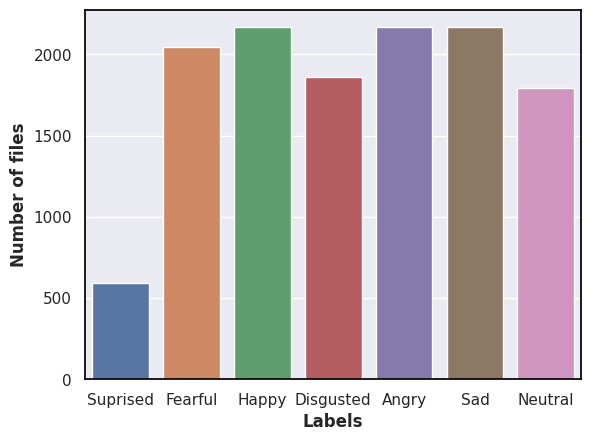
\includegraphics[width=0.8\textwidth]{cap2/images/dataset-bars.png}
    \caption{Número de audios del dataset}
    \label{fig:data-bars}
\end{figure}

% insert pie image
\begin{figure}[H]
    \centering
    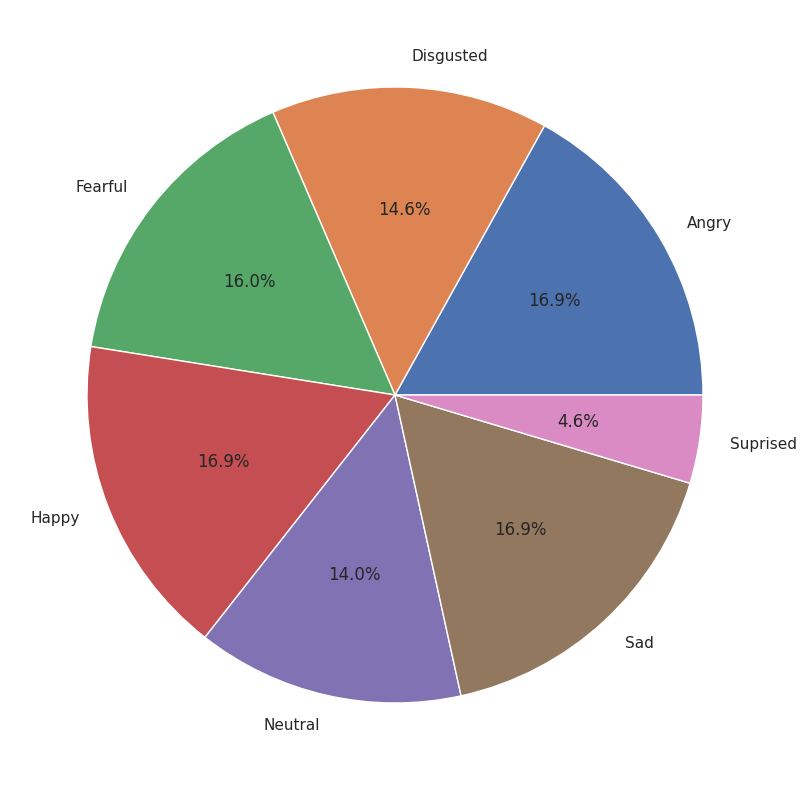
\includegraphics[width=0.8\textwidth]{cap2/images/dataset-pie.png}
    \caption{Porcentaje de audios del dataset}
    \label{fig:data-pie}
\end{figure}


El dataset contiene un total de 12.798 audios, con una duración de 3 segundos cada uno.

Echando un vistazo a la \autoref{fig:data-bars} y a la \autoref{fig:data-pie}, podemos observar un claro desbalance en la clase \textit{surprised}, que contiene un número muy inferior de audios que el resto de clases.
Como no existen restricciones en cuanto a las clases que se quieren clasificar, se ha optado por eliminar esta clase del dataset, y quedarnos con las 6 clases restantes.
De este modo se consigue un dataset más equilibrado, lo cual influirá positivamente en el entrenamiento del modelo.

\begin{figure}[H]
    \centering
    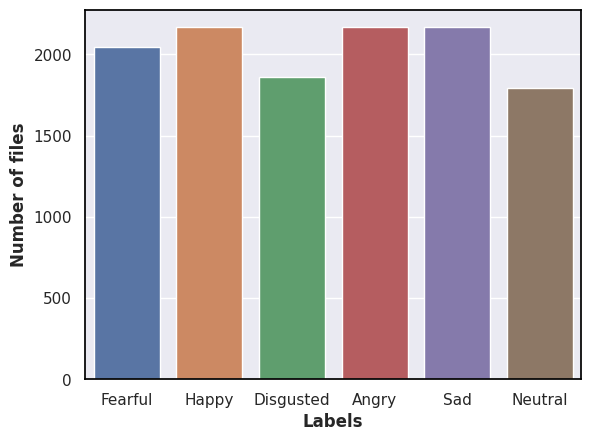
\includegraphics[width=0.8\textwidth]{cap2/images/dataset-bars-small.png}
    \caption{Número de audios del dataset reducido}
    \label{fig:data-bars-small}
\end{figure}

% insert pie image
\begin{figure}[H]
    \centering
    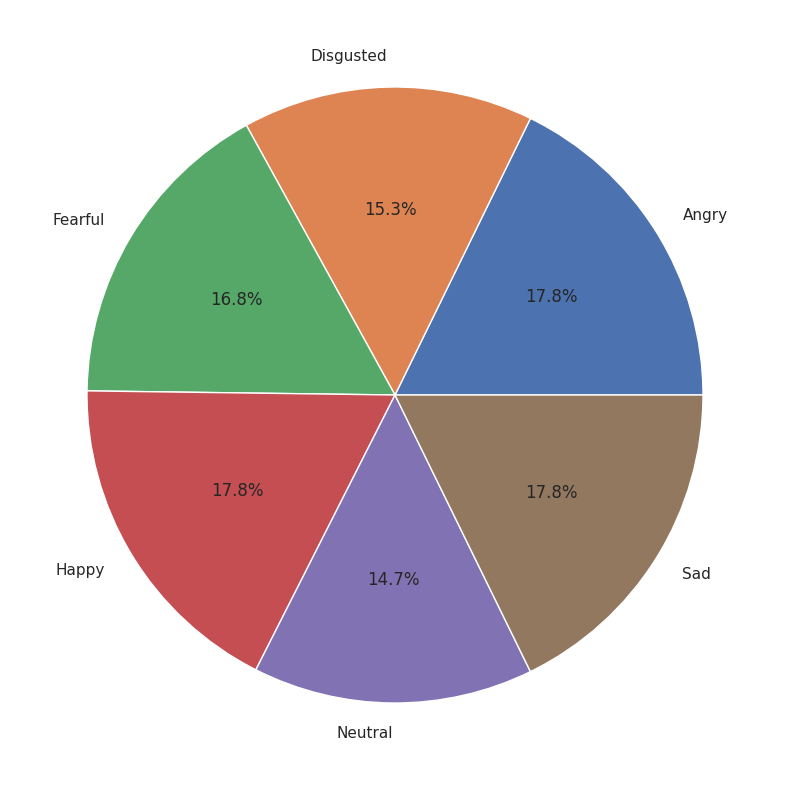
\includegraphics[width=0.8\textwidth]{cap2/images/dataset-pie-small.png}
    \caption{Porcentaje de audios del dataset reducido}
    \label{fig:data-pie-small}
\end{figure}

Esta versión del dataset cuenta con un total de 12.206 audios, con una duración de 3 segundos cada uno.

\section{Modelo}\label{seccion:modelo}
Una vez se ha seleccionado el dataset, se ha procedido a la creación del modelo.

\subsection{Estado del arte}\label{seccion:estado-del-arte}
Para poder enfocar un problema del que no se tiene conocimiento previo, es necesario realizar una investigación previa sobre el estado del arte, primero, para determinar si es posible resolver el problema, y segundo, para conocer las herramientas que existen para resolverlo.
En este caso, se ha realizado una investigación sobre las herramientas que existen para la clasificación de audios.

La solución parece estar ubicada en el campo de la \textit{Inteligencia Artificial}, y más concretamente en el campo del \textit{Deep Learning} debido a la dificultad de encontrar patrones en los audios.
Es importante saber clasificar nuestro problema dentro de un campo de la \textit{Inteligencia Artificial}, ya que existen diferentes herramientas para resolver problemas de diferentes campos.

Trabajos relacionados muestran un gran desempeño de la arquitectura conocida como \textbf{Transformers} en la clasificación de audios, ya que son capaces de capturar patrones en los audios que otras arquitecturas no son capaces de capturar.
Estos \textit{Transformers} son una arquitectura de \textit{Deep Learning} que se ha popularizado en los últimos años, y que ha demostrado un gran desempeño en la clasificación de textos y audios.
Por eso, son muy utilizados para tareas relacionadas con el campo del \textit{Natural Language Processing} (NLP), el campo del \textit{Speech Recognition} (SR), el campo del \textit{Speech Synthesis} (SS), y el campo del \textit{Emotion Recognition} (ER).

Desde que en 2017 salió a la luz el artículo \textit{Attention is all you need} \cite{vaswani2023attention}, en el que se presentaba la arquitectura \textit{Transformer}, se han realizado numerosos trabajos que han mostrado prometedores resultados en la clasificación de textos y audios. \cite{standfordCS224N} \cite{sullivan2022improving}

Sin embargo, su uso estaba reservado a grandes empresas con grandes recursos, ya que el entrenamiento de estos modelos requiere de una gran cantidad de datos y de una gran capacidad de cómputo.

Además de esto, la gran complejidad que presentaban hacía que su uso fuera muy complicado para usuarios con pocos conocimientos en el campo del \textit{Deep Learning}.
La aparición de librerías de un mayor nivel de abstracción ha acercado el uso de estas arquitecturas a usuarios con menos conocimientos.
Una de las librerías más utilizadas es \textit{Transformers}, desarrollada y mantenida por \textit{Hugging Face}, que ofrece una gran cantidad de herramientas para la carga de modelos pre-entrenados, realizar ajustes finos de estos modelos, procesar datos de entrada, etc.
Está pensado para poder ser usado por todo tipo de usuarios, desde usarios con pocos conocimientos que quieran usar modelos pre-entrenados, usuarios con conocimientos avanzados que quieran realizar un ajuste fino de los modelos pre-entrenados, hasta investigadores que quieran crear sus propios modelos. \cite{transformers-docs}


\subsection{Elección del modelo}\label{seccion:eleccion-del-modelo}
Una vez se ha realizado una investigación sobre el estado del arte, se ha decidido utilizar un modelo pre-entrenado de los disponibles en la librería \textit{Transformers}.
Esta elección no es sencilla debido a la gran cantidad de opciones disponibles y la aparente similitud entre ellas.
Para poder elegir el modelo más adecuado, se ha realizado una búsqueda sobre cuáles son los modelos más utilizados en la clasificación de audios.

Tras investigar sobre los modelos más utilizados, se ha decidido utilizar el modelo \textit{Wav2Vec2} \cite{baevski2020wav2vec}
Este modelo ha sido creado por \textit{Facebook AI} específicamente para ser utilizado en tareas de los campos de \textit{Speech Recognition} (SR) y \textit{Audio Classification}.
Además, es un modelo popular entre usuarios de la librería \textit{Transformers}, incluso cuenta con ejemplos de uso en la documentación oficial de la librería.

Por estos motivos, se ha considerado más que apropiado para la resolución del problema que se plantea en este proyecto.

También ha sido empleado otro modelo bastante más grande, el modelo \textit{XLSR-Wav2Vec2} \cite{conneau2020unsupervised}.
Es una mejora del modelo "Wav2Vec2", que ha sido entrenado con una gran cantidad de datos de diferentes idiomas.
Este modelo ha sido utilizado para la clasificación de audios en diferentes idiomas, y se ha considerado interesante probarlo para la clasificación de audios en español.
La elección de este modelo se ha realizado con la finalidad de mejorar los resultados obtenidos con el modelo "Wav2Vec2", ya que es un modelo más versátil para la clasificación de audios en diferentes idiomas. \cite{greekEmotionRecognition}
Sin embargo, al ser más complejo requeriría una mayor capacidad de cómputo para su entrenamiento, además de un mejor ajuste de los parámetros.
Al no obtener mejores resultados que el modelo "Wav2Vec2", siendo más exigente computacionalmente, se ha decidido no utilizarlo en la solución final.


\section{Entrenamiento}\label{seccion:entrenamiento}
Una vez se ha seleccionado el modelo, se ha procedido a realizar el entrenamiento del mismo.

\subsection{Preparación del entrenamiento}\label{seccion:preparacion-del-entrenamiento}
Antes de comenzar el entrenamiento del modelo, es necesario realizar una serie de preparaciones previas.
La siguiente elección consiste en decidir qué librería de bajo nivel se va a utilizar para el entrenamiento del modelo.
\textit{Transformers} ofrece una documentación muy extensa con multitud de ejemplos en muhos campos, y dentro de estos ejemplos, podemos elegir entre \textit{PyTorch} y \textit{TensorFlow}, dos librerías de bajo nivel muy populares en el campo del \textit{Deep Learning}.

En principio no debe existir diferencia entre utilizar una u otra, ya que ambas librerías ofrecen las mismas funcionalidades.
Dependerá de la experiencia del usuario con una u otra, o de la preferencia del usuario.
En este caso, se ha optado por utilizar \textit{PyTorch}, ya que es una librería con la que se tiene algo más de experiencia, y además, es la librería que se utiliza en la documentación oficial de \textit{Transformers}.
Para un caso de uso en el que se requiera una mayor optimización de la solución, convendría estudiar más en profundidad las diferencias entre ambas librerías, y elegir la que mejor se adapte a las necesidades del usuario.

Una vez se ha elegido la librería de bajo nivel, se ha procedido a la preparación de los datos de entrada.
Los datos son en primer lugar descargos en una carpeta local.
Esta tarea es sencilla ya que \textit{Kaggle} permite cargar automáticamente los datos desde un script de Python.

Los datos no pueden ser introducidos directamente en la red neuronal, ya que esta espera recibir los datos en un formato específico.
Para esto, el modelo ofrece una herramienta que se encarga de procesar los datos de entrada y convertirlos en el formato que espera recibir la red neuronal.

El preprocesado de los datos, se basa en los siguientes pasos:
\begin{enumerate}
    \item Descarga de los datos desde Kaggle.
    \item Descarte de la clase \textit{surprised}.
    \item Creación de un dataframe con los datos descargados.
    \item Conversión a objeto interpretable por la librería de Hugging Face.
    \item Mezcla de los datos y división en conjunto de entrenamiento y conjunto de test.
    \item Codificación de las etiquetas.
    \item Preparación del Feature Extractor de nuestro modelo.
    \item Procesado de los datos de entrada (frecuencia de muestreo y duración).
    
\end{enumerate}

\begin{lstlisting}[language=Python, caption=Preprocesado del dataset, label={code:download-data}]
# download dataset
import opendatasets as od
od.download("https://www.kaggle.com/datasets/uldisvalainis/audio-emotions")

df=pd.DataFrame(glob('audio-emotions/Emotions/*/*.wav'),columns=['paths'])

df['labels']=df.paths.apply(lambda x:x.split('/')[-2])

# drop rows where label is 'Surprised'
df=df[df.labels!='Suprised']


hf_data=datasets.Dataset.from_pandas(df)
hf_data=hf_data.class_encode_column("labels")#convert label to HF label class

hf_data=hf_data.train_test_split(train_size=0.8,seed=0)

# Create a dictionary that maps a label name to an integer and vice versa. The mapping will help the model recover the label name from the label number:
labels = hf_data['train'].features['labels'].names
label2id, id2label = dict(), dict()
for i, label in enumerate(labels):
    label2id[label] = str(i)
    id2label[str(i)] = label

#feature extractor
from transformers import AutoFeatureExtractor
model='facebook/wav2vec2'
feature_extractor = AutoFeatureExtractor.from_pretrained(model)

#process the data such as fix sample rate
hf_data = hf_data.cast_column("paths", datasets.Audio(sampling_rate=16_000))

def preprocess_function(examples):
    audio_arrays = [x["array"] for x in examples["paths"]]
    inputs = feature_extractor(
        audio_arrays, sampling_rate=feature_extractor.sampling_rate, max_length=16000*2, truncation=True
    )
    return inputs


encoded_dataset = hf_data.map(preprocess_function, remove_columns=["paths"], batched=True)


\end{lstlisting}

% \medskip


\subsection{Entrenamiento del modelo}\label{seccion:entrenamiento-del-modelo}
Una vez se ha realizado el preprocesado de los datos, como se muestra en el \autoref{code:download-data}, podemos entrenar el modelo.

Debemos definir ahora la métrica que vamos a utilizar para evaluar el desempeño del modelo.
De este modo podremos calcular lo bien o mal que se comporta el modelo durante el entrenamiento, y así ir ajustando los pesos.

En este caso, se ha optado por utilizar la métrica \textit{accuracy}, que define la proporción de predicciones correctas realizadas por el modelo.
Para esta tarea, de nuevo, existe una librería de \textit{Hugging Face} que facilita la integración de esta métrica en el entrenamiento del modelo.

En este punto, podemos comenzar el entrenamiento del modelo.
La librería \textit{Transformers} permite guardar checkpoints del modelo durante el entrenamiento, de modo que podemos parar el entrenamiento en cualquier momento y continuar desde el último checkpoint guardado.
Una vez completado el entrenamiento, subiremos la mejor versión del modelo a la plataforma \textit{Hugging Face} para poder utilizarlo en producción.
De este modo nos aseguramos de que el modelo va a estar disponible en cualquier momento, y podemos compartirlo con otros usuarios, además de las ventajas que ofrecen los sistemas de control de versiones.

Los requisitos de seguridad de un proyecto real podrían requerir que el modelo no estuviera disponible públicamente, por lo que se debería buscar una alternativa para compartir el modelo con otros usuarios.
Como no es objetivo de este proyecto profundizar en este aspecto, se ha optado por aprovechar las ventajas de utilizar los servicios gratuitos que ofrece \textit{Hugging Face}.

El modelo desarrollado se encuentra disponible en la plataforma \textit{Hugging Face} guardado con el nombre de \textit{antonjaragon/emotions\_6\_classes\_small} donde se muestran los resultados, y podemos probar el modelo con audios de prueba.
Por otro lado, aunque no ha sido utilizado en este trabajo, también existe el modelo entrenado con el modelo \textit{XLSR-Wav2Vec2}, guardado con el nombre de \textit{antonjaragon/emotions\_6\_classes}.

En el \textbf{\href{https://huggingface.co/antonjaragon/emotions_6_classes_small}{repositorio}} se puede acceder a información más detallada sobre el entrenamiento del modelo, y se puede probar el modelo con audios de prueba.


\begin{lstlisting}[language=Python, caption=Entrenamiento del modelo, label={code:train-model}]

import evaluate
accuracy = evaluate.load("accuracy")

def compute_metrics(eval_preds):
    # metric = datasets.load_metric("accuracy")
    logits, labels = eval_preds
    predictions = np.argmax(logits, axis=1)
    return accuracy.compute(predictions=predictions, references=labels)

from transformers import AutoModelForAudioClassification, TrainingArguments, Trainer

num_labels = len(id2label)
model = AutoModelForAudioClassification.from_pretrained(model, num_labels=num_labels, label2id=label2id, id2label=id2label)

training_args = TrainingArguments(
    output_dir="./emotions",
    evaluation_strategy="epoch",
    save_strategy="epoch",
    fp16=True,
    learning_rate=3e-5,
    per_device_train_batch_size=32,
    gradient_accumulation_steps=4,
    per_device_eval_batch_size=32,
    num_train_epochs=10,
    warmup_ratio=0.1,
    logging_steps=10,
    load_best_model_at_end=True,
    metric_for_best_model="accuracy",
    push_to_hub=True,

)

trainer = Trainer(
    model=model,
    args=training_args,
    train_dataset=encoded_dataset['train'],
    eval_dataset=encoded_dataset["test"],
    tokenizer=feature_extractor,
    compute_metrics =compute_metrics,

)

trainer.train()

\end{lstlisting}


Las posibilidades de la librería \textit{Transformers} son muy amplias, y permiten realizar ajustes finos del modelo, como por ejemplo, la posibilidad de utilizar diferentes optimizadores, diferentes funciones de pérdidas, diferentes métricas, etc.
Esto permite que el usuario pueda ajustar el modelo a sus necesidades, y pueda realizar un entrenamiento más eficiente.

En este caso, se ha optado por utilizar las opciones por defecto, e intentar mejorar resultados modificando algunos parámetros como el ratio de aprendizaje o el número de épocas de entrenamiento.
Al ser un procesamiento muy costoso, no se ha podido profundizar mucho en este aspecto, pero se ha conseguido un modelo que ofrece una funcionalidad básica.

Los resultados obtenidos por el mejor modelo son los siguientes:
\begin{itemize}
    \item \textbf{Accuracy}: 0.7920
    \item \textbf{Loss}: 0.9106
\end{itemize} 



\section{Saturn Cloud}\label{seccion:saturn-cloud}
Para el entrenamiento del modelo, se ha hecho uso de los recursos gratuitos que ofrece la plataforma \textit{Saturn Cloud}.

El proceso de entrenamiento de un modelo de \textit{Deep Learning} es muy costoso computacionalmente, y requiere de una gran capacidad de cómputo.
Las primeras pruebas se realizaron en un portátil personal con una tarjeta gráfica integrada.

Realizar entrenamientos pesados de varias horas de duración no es viable para un ordenador personal, ya que el desgaste sería muy elevado.
Por ello, se han buscado alternativas a probar en este proyecto en concreto.
Utilizar servicios de terceros para el entrenamiento de modelos puede no ser viable en muchos casos, debido a que necesitamos cargar los datos en la nube.
Esto puede ser un problema si los datos son sensibles, ya que no podemos garantizar la seguridad de los mismos.
Sin embargo, al estar utilizando un dataset público, no es un problema cargar los datos en el servidor de entrenamiento.

Además, el coste de utilizar estos servicios puede ser muy elevado, ya que el entrenamiento de un modelo puede durar varias horas, y el coste se calcula en función del tiempo de uso de los recursos.
Esta solución no sería la mejor para muchos escenarios, pero en este caso, se ha optado por utilizar los recursos gratuitos que ofrece la plataforma \textit{Saturn Cloud}.
La elección se debe a que es una de las pocas plataformas que ofrecen una instancia con GPU en el segmento gratuito.
Para nuevos usuarios, contamos con 150 horas de uso de una instancia con GPU, que es más que suficiente para realizar varios entrenamientos del modelo.

Este tipo de plataformas están directamente enfocadas al entrenamiento de modelos de \textit{Deep Learning}, por lo que ofrecen una gran cantidad de herramientas para facilitar el entrenamiento de modelos.
Existe multitud de imágenes pre-configuradas con las herramientas más utilizadas, y además, ofrecen la posibilidad de crear imágenes personalizadas con las herramientas que necesitemos.
En concreto, se han utilizado imágenes \textit{Debian} con \textit{PyTorch} pre-instalado.

\begin{figure}\label{fig:saturn-cloud}
    \centering
    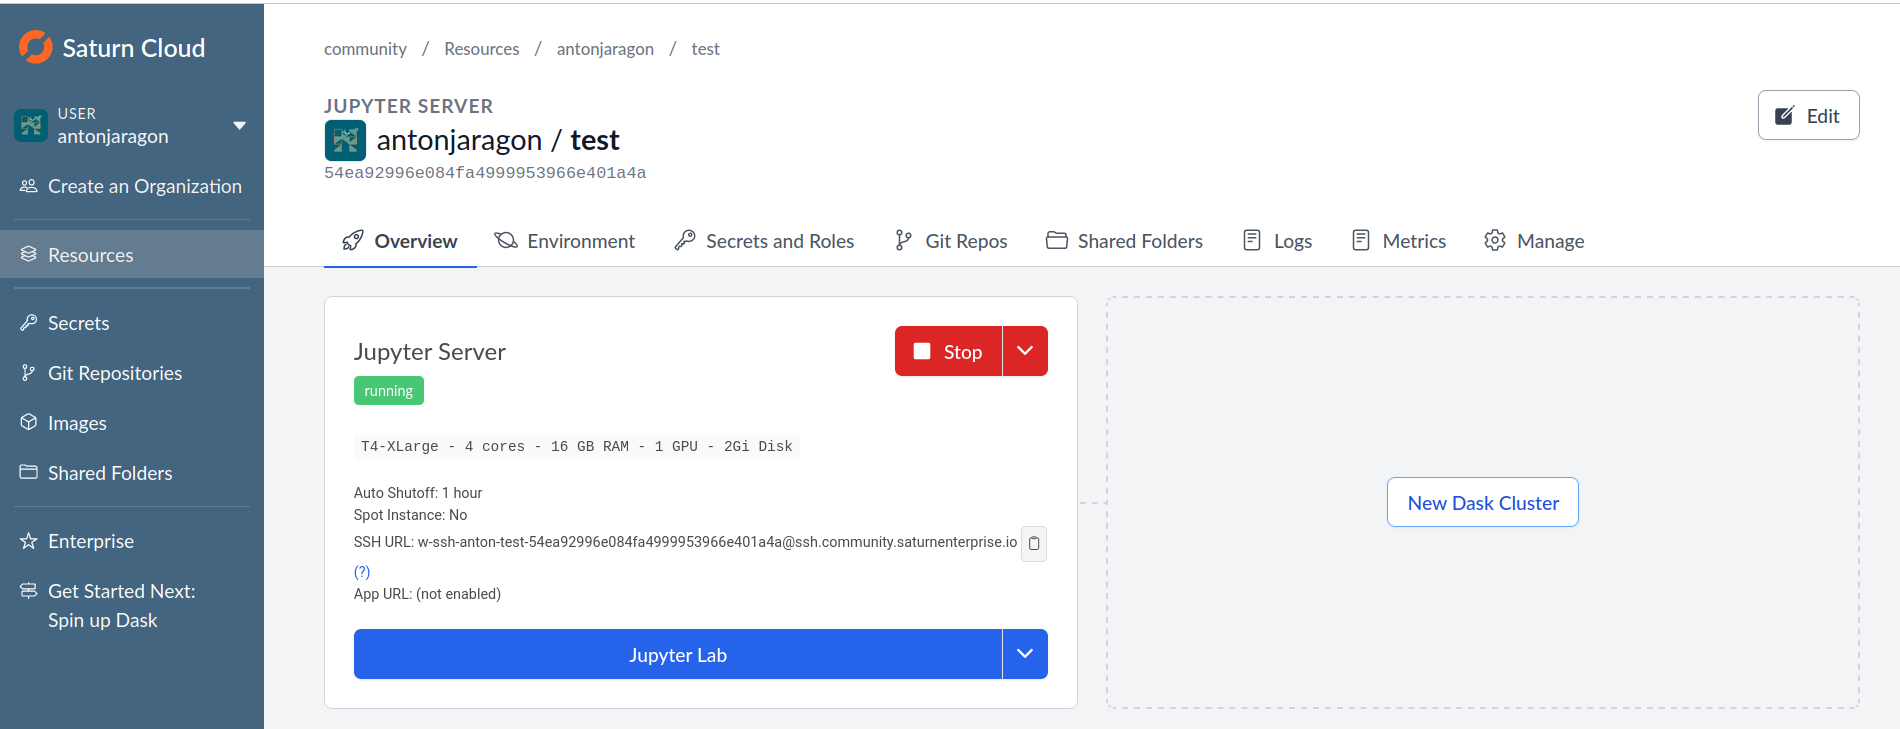
\includegraphics[width=0.8\textwidth]{cap2/images/saturn-cloud.png}
    \caption{Ejemplo de instancia activa con GPU en Saturn Cloud}
    
\end{figure}



\endinput%Creación del modelo
% 
\chapter{Despliegue del modelo}\label{chp-03}
\epigraph{Less is more.}{Ludwig Mies van der Rohe}

\section{Problemática y solución}

Nos encontramos en esta situación: el modelo ha sido entrenado o está siendo desarrollado por otro equipo.
Nuestro trabajo consiste en implementarlo en un entorno de producción para que pueda ser utilizado por los usuarios finales.

Este problema puede ser abordado de varias formas, y la solución estará altamente condicionada por los requisitos del proyecto.
Al no tener ningún requisito impuesto para este trabajo, surgen muchos interrogantes cuya respuesta no es trivial:

\begin{itemize}
    \item \textbf{Aspecto final de la solución}: ¿Cómo se va a utilizar el modelo? ¿Qué tipo de interfaz se va a utilizar? ¿Qué tipo de dispositivo se va a utilizar?
    \item \textbf{Requisitos de la solución}: ¿Qué requisitos de rendimiento tiene la solución? ¿Qué requisitos de seguridad tiene la solución? ¿Qué requisitos de escalabilidad tiene la solución?
    \item \textbf{Arquitectura de la solución}: ¿En qué lenguaje se va a implementar la solución? ¿Qué tipo de arquitectura se va a utilizar? ¿Qué tipo de servidores se van a utilizar?
    
\end{itemize}

En este caso, se ha optado por simplificar el aspecto final de la solución para centrarnos en la implementación del modelo en un entorno de producción.
Se ha decidido crear una interfaz web que permita a los usuarios finales interactuar con el modelo, y una implementación mediante contenedores Docker para facilitar el despliegue en cualquier entorno.

\section{Enfoque escogido}
En un principio se pensó en realizar inferencia en tiempo real, es decir, que la aplicación, una vez iniciada, estuviera grabando continuamente y realizando predicciones.
Esta opción sin embargo, no ha podido ser llevada a cabo de forma exitosa debido al tiempo de respuesta que ofrece el servidor en el que se ha desplegado la aplicación.

Además, para implementarlo de forma correcta, habría que añadir diversos mecanismos que ayuden a filtrar los audios y nos permitieran extraer muestras que pudieran ser utilizadas para realizar predicciones.
Esto implicaría detección de inicio y fin de actividad vocal, filtrado de silencios, etc.
La complicación de este proceso, unido al tiempo de respuesta del servidor, ha hecho que se descarte esta opción.

Finalmente, contamos con una aplicación web que permite a los usuarios finales grabar audios y obtener una predicción de la clase a la que pertenece el audio.
La aplicación está pensada para ser utilizada en una sola dirección: el usuario debe iniciar la grabación, grabar un mensaje, parar la grabación y esperar el resultado.
Una vez obtenido el resultado, puede volver a grabar otro mensaje.

La aplicación es accesible desde cualquier dispositivo que tenga un navegador web a través de la dirección \url{https://www.classifier-web.com/}.


\section{Aplicación web}
Una forma sencilla de crear una interfaz que sea accesible desde cualquier dispositivo es crear una aplicación web.

Aunque el modelo creado puede ser integrado utilizando cualquier lenguaje de programación, se ha optado por utilizar Python para la implementación de la aplicación web.
Python cuenta con una gran cantidad de librerías que facilitan la implementación de aplicaciones web, como Flask o Django, quizás las más populares.

Se ha optado por utilizar Flask, debido a que es una librería más ligera que Django y a que es más sencilla de utilizar.
Además, contamos con cierta experiencia previa en el uso de Flask, lo que nos permite acelerar el desarrollo de la aplicación.


\subsection{Flask}
Flask es un microframework para Python que permite crear aplicaciones web de forma sencilla.

Está diseñado para ser extensible, por lo que es posible añadirle funcionalidades mediante extensiones, aunque en este caso no vamos a utilizar ninguna.
Sin embargo, estas extensinoes de alto nivel nos abren las puertas a posibles líneas futuras, como lecturas de bases de datos, autenticación de usuarios, etc.

Utilizar Python para la creación web no siempre es la solución idónea, ya que existen otros lenguajes de programación que están más orientados a la creación de aplicaciones web.
Sin embargo, si no se tiene experiencia previa en estos lenguajes, o el objetivo es lanzar una aplicación web de forma rápida, Flask es idóneo.
No estamos exentos de tener que crear plantillas en otros lenguajes propios de la web, como HTML, CSS o JavaScript, pero Flask nos permite crear una aplicación web funcional en muy poco tiempo.


\subsection{Estructura de la aplicación}
La estructura de la aplicación es muy sencilla, y se puede ver en la figura """poner figura""""

Primero el modelo es cargado en memoria, y se crea una instancia de Flask.

El modelo es cargado en memoria para evitar tener que cargarlo cada vez que se realiza una predicción, lo que se traduciría en un aumento del tiempo de respuesta de la aplicación.
Esto puede ralentizar sin embargo el arranque de la aplicaión, pero es una operación que se realiza una única vez, por lo que no es un problema.

Posteriormente se crean las rutas de la aplicación, que son las direcciones a las que se puede acceder desde un navegador web.

Contamos con la ruta principal, que es la que se utiliza para cargar la página principal de la aplicación, y la ruta de predicción, que es la que se utiliza para realizar las predicciones.

La ruta principal simplemente carga un fichero HTML que contiene el código de la página principal.

La ruta de predicción es llamada internamente mediante una petición POST cuando un usuario termina una grabación.
La grabación se guarda localmente en el servidor momentáneamente para que el modelo pueda realizar la predicción sobre ella, y posteriormente se borra, por cuestiones de espacio y privacidad.



\subsection{Interfaz web}
El desarrollo de interfaces web es un mundo aparte, y no es el objetivo de este trabajo crear una interfaz especialmente atractiva, sino más bien que nos proporcione la funcionalidad básica.
Existen desarrolladores especializados únicamente en el desarrollo de interfaces web, y es un campo que requiere de un conocimiento muy amplio, además de experiencia.

Debido a tratar esta parte como algo secundario, sumado a la falta de conocimiento acerca del manejo de audios en la web, se ha optado por basar la interfaz en trabajo previo realizado por otros desarrolladores.
En concreto, este proyecto ha utilizado como base """insertar referencia a la interfaz web""".

La interfaz web es muy sencilla, y se puede ver en la figura """poner figura""". 
Contiene lo básico para que un usuario pueda realizar la grabación de un audio y obtener una predicción de la clase a la que pertenece el audio.



\section{Aplicación Flask en producción}
Flask integra un servidor web de desarrollo, que es el que se utiliza por defecto cuando se lanza la aplicación, llamado Werkzeug.
Este servidor es muy sencillo de utilizar, pero no está pensado para ser utilizado en producción, ya que no está optimizado para ello.


\subsection{Gunicorn}
Para lanzar la aplicación en producción, se ha optado por utilizar Gunicorn, un servidor web HTTP WSGI para Python.
Es uno de los servidores más utilizados para lanzar aplicaciones Flask en producción, y es el que se recomienda en la documentación oficial de Flask.??????????????

Gunicorn es un servidor web que se encarga de gestionar las peticiones HTTP que llegan a la aplicación, y de lanzar procesos de la aplicación para atender estas peticiones.
Esto permite que la aplicación pueda atender varias peticiones simultáneamente, lo que se traduce en un aumento del rendimiento de la aplicación.

Para lanzar un servicio Flask con Gunicorn, simplemente hay que ejecutar el siguiente comando:
""" Insertar comando """"

Este comando lanzará un servidor web en el puerto 8000, que es el puerto por defecto de Gunicorn.

El siguiente paso es configurar un servidor web que actúe como proxy inverso, para que las peticiones HTTP que lleguen al servidor web sean redirigidas al servidor Gunicorn.


\subsection{Traefik}
Para configurar el servidor web que actúe como proxy inverso, se ha optado por utilizar Traefik, un servidor web que permite realizar balanceo de carga y que actúa como proxy inverso.

Aunque Nginx es quizás el servidor web más utilizado para realizar esta tarea, se ha optado por utilizar Traefik prinipalmente por su facilidad de configuración.
Es comentado que Nginx es más rápido que Traefik, a la vez que ofrece más funcionalidades, pero para este caso con una configuración básica es suficiente.

La mayor ventaja que nos ha brindado Traefik es la facilidad de generar certificados SSL para la aplicación, lo que nos permite utilizar HTTPS.
Esto es importante, ya que si no se utiliza HTTPS, los navegadores web no permiten acceder al micrófono del dispositivo, lo que hace imposible la grabación de audios.

No es una tarea difícil de realizar correctamente para un desarrollador experimentado mediante un servidor web como Nginx, pero es mucho más sencillo de realizar con Traefik, y además, al contar con poca experiencia en este campo, nos ha permitido solventar este problema de forma rápida y sencilla.
Además, Traefik aún está dando sus primeros pasos, y está ganando popularidad entre desarrolladores, por lo que quizás en un futuro sea una alternativa a Nginx también en entornos reales de producción.

""" insertar foto de \url{https://monitor.classifier-web.com} indicando admin:admin"""

\subsection{Docker}
Para facilitar el despliegue de la aplicación en cualquier entorno, se ha optado por utilizar contenedores Docker.
Esta tecnología permite encapsular una aplicación y sus dependencias en un contenedor, que puede ser ejecutado en cualquier entorno que tenga instalado Docker.
De este modo nos aseguramos que únicamente tenemos que preocuparnos de que el entorno tenga instalado Docker.

Esta tecnología ayuda a eliminar muchos problemas a la hora de desplegar servicios, pero incorpora otros de los que hay que ser conscientes.
En particular, Docker presenta un problema de seguridad, ya que los contenedores son ejecutados por defecto con privilegios de root.
Esto implicaría que si un atacante consigue acceder al contenedor, puede tener acceso a todo el sistema.

Este problema se ha solventado creando un usuario no privilegiado dentro del contenedor al construir la imagen de la aplicación, y ejecutando la aplicación con este usuario.
Sin embargo, las implicaciones de seguridad de Docker son un tema muy amplio y precisamente pueden llegar a ser determinantes para no utilizar esta tecnología en entornos de producción con requisitos de seguridad muy estrictos.
No es el caso de este trabajo, pero es un tema que hay que tener en cuenta y debería ser estudiado en profundidad antes de utilizar Docker en entornos de producción.

A pesar de ello, las ventajas que ofrece Docker son muy interesantes, y es una tecnología que ha ganando mucha popularidad en los últimos años.
Las principales ventajas que ofrece son las siguientes:

\begin{itemize}
    \item \textbf{Portabilidad}: Docker permite encapsular una aplicación y sus dependencias en un contenedor, que puede ser ejecutado en cualquier entorno que tenga instalado Docker.
    \item \textbf{Escalabilidad}: Docker permite crear múltiples contenedores de una misma aplicación, lo que permite escalar la aplicación de forma horizontal.
    \item \textbf{Aislamiento}: Docker permite aislar una aplicación y sus dependencias en un contenedor, lo que permite que la aplicación no se vea afectada por otras aplicaciones que se estén ejecutando en el mismo entorno.
    \item \textbf{Rapidez}: Docker permite crear imágenes de aplicaciones de forma rápida, lo que permite desplegar aplicaciones en muy poco tiempo.
\end{itemize}

\subsection{Docker Compose}
Docker Compose es una herramienta que permite definir y ejectutar aplicaciones Docker de forma sencilla.
Permite definir las imágenes de los contenedores, las redes, los volúmenes, etc., en un fichero YAML, y ejecutarlos con un único comando.

Es especialmente útil cuando se tienen varias aplicaciones que dependen unas de otras, ya que permite definir todas las aplicaciones en un único fichero.
En nuestro caso contamos solo con dos contenedores, pero crear un fichero Docker Compose nos permite definirlos de forma sencilla, construir las imágenes con las dependencias que nosotros definamos y levantar el despliegue con un único comando.

""" enlace a codigo de anexo """

\section{Plataforma de hosting}
- Hablar de Aws
- VPS Contabo: precio fijo



\endinput%Despliegue del modelo
%

\chapter{Conclusiones}\label{chp-04}

% quote from Einstein
\epigraph{If we knew what it was we were doing, it would not be called research, would it?}{Albert Einstein}

\lettrine[lraise=-0.1, lines=2, loversize=0.2]{U}{na} vez finalizado el proyecto, es momento de hacer una valoración del mismo. 
En este capítulo se exponen las conclusiones obtenidas tras la realización del proyecto, así como las posibles mejoras que se podrían realizar en un futuro.

\section{Cumplimiento de requisitos}
Después de haber estado enfocado en un proyecto exigente durante un periodo de tiempo prolongado, tener sentimientos encontrados es normal. 
Pensar que se podrían haber realizado más pruebas, o que se podría haber mejorado algún aspecto, es inevitable.

Sin embargo, hay que echar la vista atrás y ver de dónde venimos para entender el camino recorrido.
El objetivo principal del proyecto, que era crear y desplegar un modelo clasificador de audios ha sido cumplido.

Para entender el grado de éxito del proyecto, es necesario recordar los requisitos que se establecieron en el capítulo \ref{chp-02} y ver cuáles de ellos se han cumplido.

\subsubsection{Requisitos funcionales}
Se han cumplido todos los requisitos funcionales.
El modelo es capaz de clasificar audios de entrada en formato WAV, y el sistema es accesible desde cualquier navegador web.
Además, el proceso de entrenamiento es replicable, y se puede entrenar un nuevo modelo con nuevos datos.

No se determinó ningún porcentaje de acierto mínimo, pero esta característica sería algo normal en un proyecto de estas características.

\subsubsection{Requisitos operacionales}
Debido a la falta de pruebas exhaustivas, no se puede asegurar que el sistema cumpla los requisitos operacionales con un alto grado de confianza.
Por ejemplo, es accesible desde cualquier y en cualquier momento, pero no se ha realizado un estudio de la disponibilidad del sistema.

Tampoco sabemos cómo puede comportarse el sistema con una carga de trabajo elevada.
Queda pendiente para líneas futuras la elaboración de un estudio de rendimiento del sistema y verificación de los requisitos operacionales.

\subsubsection{Requisitos de diseño}
El sistema cumple con los requisitos de diseño establecidos.

Estos requisitos fueron establecidos conociendo la tecnología que se iba a utilizar, por lo que no ha habido ningún problema en este aspecto.
Sin embargo, en un proyecto real, el diseño deberá adaptarse al entorno en el que se vaya a desplegar el sistema y a las tecnologías disponibles.

\subsubsection{Requisitos de seguridad}
El sistema cumple el requisito \textbf{S.2}, ya que el servidor web utiliza el protocolo HTTPS para asegurar la comunicación con el cliente.

Sin embargo, al realizar el entrenamiento del modelo en una instancia remota, no se ha podido cumplir el requisito \textbf{S.1}.
Además, para garantizar la seguridad del sistema, sería necesario realizar un estudio de las vulnerabilidades del mismo.



\section{Lecciones aprendidas}
El aprendizaje adquirido durante el desarrollo del proyecto ha sido muy valioso.
Más allá de las cuestiones puramente técnicas, se han adquirido múltiples habilidades que serán de gran utilidad en el futuro.

El hecho de enfocar el proyecto como un problema real, obliga a imaginarse qué tipo de problemas pueden surgir y qué elección es la más adecuada para resolverlos.
Aunque muchos requisitos han sido obviados, sobre todo los relacionados con la seguridad, entender las implicaciones que tienen las decisiones tomadas es muy enriquecedor.

Quizás el mayor aprendizaje ha sido el relacionado con cómo los obstáculos han sido sorteados.
Es inevitable que surjan problemas durante el desarrollo de un proyecto, y muchos de ellos parecen bloquear el avance.
Sin embargo, es en estos puntos cuando hay que entender bien el problema para poder encontrar una solución, o un camino alternativo.

En relación con el previo acercamiento a esta problemática, muchos de estos obstáculos que antes bloqueaban el proyecto por completo, han podido ahora ser resueltos o evitados.
En esta línea, es importante entender que muchas veces la solución no es un camino recto, sino que a veces hay que tomar desvíos para poder llegar al destino.


\section{Líneas futuras}

Esta sección pretende servir de autocrítica y de guía para futuros proyectos que quieran continuar con el trabajo realizado.
Se van a enumerar los puntos que se consideran más importantes para mejorar el proyecto.


\subsection{Mejorar el modelo}
A pesar de contar con un modelo capaz de clasificar audios, hemos comprobado que los resultados pueden ser mejorables.
En particular, sería conveniente prestar atención a las clases más problemáticas para subir el porcentaje de acierto.

Para ello, se podrían realizar las siguientes acciones:
\begin{itemize}
    \item Aumentar el número de muestras de las clases más problemáticas.
    \item Ajustar parámetros de entrenamiento.
    \item Probar distintos modelos preentrenados.
    \item Probar técnicas de Data Augmentation.
\end{itemize}




\subsection{Añadir funcionalidad al sistema}
% Explicar que solo hace una cosa
Otro punto particularmente débil de la implementación final del sistema es que tiene una funcionalidad muy limitada.
El sistema es capaz de clasificar audios de entrada que se suponen válidos, pero nada más.

Sería interesante añadir funcionalidades que permitan al usuario interactuar con el sistema de forma más natural.
Por ejemplo, grabar de forma continua y detectar emociones dependientes del tiempo.
Esta nueva funcionalidad no se consigue simplemente grabando de forma continua y haciendo predicciones, sería conveniente añadir un bloque detector de actividad vocal.

Una posible futura mejora podría ser un sistema capaz de detetar palabras clave. 
El desarrollo de este tipo de sistemas es muy similar al de los clasificadores de emociones, pero se necesitaría un dataset de grabaciones de la palabra clave en cuestión.
Acompañado de un estudio de las palabras clave que pudieran resultar de interés, este nuevo sitema podría ser de gran utilidad al clasificador de emociones.

También se podría investigar cómo identificar el hablante.
Hasta el momento hemos supuesto que hay un solo hablante, pero en caso de que hubiera más de uno, sería interesante identificarlos para poder obtener información temporal de cada uno de ellos.


\subsection{Verificación de funcionamiento}
La verificación del funcionamiento de un sistema puede llegar a consumir la mayor parte del tiempo de desarrollo.
En proyectos cuya disponibilidad es crítica, o se necesita un alto grado de confianza en el sistema, es necesario realizar una verificación exhaustiva del mismo.

Asegurar que el sistema no va a fallar es muy complejo, y requiere de un estudio profundo de los posibles casos de uso.

Para nuestro caso de uso, la evaluación del modelo debe ser mucho más exhaustiva, contando con un dataset de test mucho más variado (audios en varios idiomas, con ruido de fondo, audios de baja calidad, audios sin palabras, grabaciones genuinas, etc.).

En cuanto al servidor web, se debería realizar una verificación de la disponibilidad del sistema, pruebas de carga, pruebas de seguridad, etc.

En este proyecto, se ha realizado una verificación básica del funcionamiento del sistema, pero no se ha profundizado en ella.



\subsection{Optimización de la solución}
Reducir los recursos necesarios que necesita el sistema es siempre algo positivo.
No sirve de nada un modelo con un 99\% de acierto si necesita más del tiempo crítico para realizar la predicción.

Por ello, paralelamente a buscar la mejor solución, en un proyecto real sería necesario balancear la solución con los recursos disponibles.

En caso de faltar recursos para realizar la predicción, se podría barajar la implementación de una solución 'b' que sea menos precisa pero más rápida.

La aplicación también debe ser optimizada según el número de usuarios que se espera que la utilicen.
En caso de que el número de usuarios sea muy elevado, se debería estudiar la posibilidad de utilizar un servidor más potente, o incluso utilizar varios servidores en paralelo.
El uso de contenedores facilita esta tarea, ya que se podrían desplegar instancias del servidor web en varios servidores y balancear la carga entre ellos.





\endinput
% 
%:Empezamos con los apéndices, que irían en uno o más ficheros. Es necesario incluir estos ficheros entre el entorno \begin{appendices}....\end{appendices} debido a que se ha deseado utilizar un formato diferente para el título de los apéndices, incluyendo la palabra apéndice, para la numeración de los apéndices, alfabético, y para las cabeceras de las páginas.

% \begin{appendices}

% % Fichero en el que se incluyen los apéndices
% % !TEX root =../LibroTipoETSI.tex



%APENDICE A
\chapter{Sobre  \LaTeX}\LABAPEN{ApA}
{Este es un ejemplo de apéndices, el texto es únicamente relleno, para que el lector pueda observar cómo se utiliza}
%%%%%%%%%%%%%%%%%
\section{Ventajas de \LaTeX}

El gusto por el \LaTeX\ depende de la forma de trabajar de cada uno. La principal virtud es la facilidad de formatear cualquier texto y la robustez. Incluir títulos, referencias es inmediato.
%\Blindtext
%\lipsum
Las ecuaciones quedan estupendamente, como puede verse en \EQ{Ap1}
\begin{equation}\LABEQ{Ap1}
x_{1}=x_{2}.
\end{equation}


\section{Inconvenientes}
%\Blindtext
El principal inconveniente de \LaTeX\ radica en la necesidad de aprender un conjunto de comandos para generar los elementos que queremos. Cuando se está acostumbrado a un entorno ``como lo escribo se obtiene'', a veces resulta difícil dar el salto a ``ver'' que es lo que se va a obtener con un determinado comando. 

Por otro lado, en general será muy complicado cambiar el formato para desviarnos de la idea original de sus creadores. No es imposible, pero sí muy difícil. Por ejemplo, con la sentencia siguiente:
 
\begin{lstlisting}[language=,caption={Escritura de una ecuación}, breaklines=true, label=prgA1-01]
\begin{equation}\LABEQ{Ap2}
x_{1}=x_{2}
\end{equation}
\end{lstlisting}
obtenemos:
\begin{equation}\LABEQ{Ap2}
x_{1}=x_{2}
\end{equation}
Esto será siempre así. Aunque, tal vez, esto podría ser una ventaja y no un incoonveniente.

Para una discusión similar sobre el Word\tsp{\textregistered}, ver \APEN{ApB}.
%\Blindtext


%%%%%%%%%%%%%%%%%%%%%%%%%%%%%%%%%%%%%%%
%APENDICE B
\chapter{Sobre Microsoft Word\tsp{\textregistered}}\LABAPEN{ApB}

\section{Ventajas del Word\tsp{\textregistered}}
La ventaja mayor del Word\tsp{\textregistered} es que permite configurar el formato muy fácilmente. Para las ecuaciones,
\begin{equation}
x_{1}=x_{2},
\end{equation}
tradicionalmente ha proporcionado pésima presentación. Sin embargo, el software adicional Mathtype\tsp{\textregistered} solventó este problema, incluyendo una apariencia muy profesional y cuidada. Incluso permitía utilizar un estilo similar al \LaTeX\xspace. Además, aunque el Word\tsp{\textregistered} incluye sus propios atajos para escribir ecuaciones,  Mathtype\tsp{\textregistered} admite también escritura \LaTeX\xspace. En las últimas versiones de Word\tsp{\textregistered}, sin embargo, el formato de ecuaciones está muy cuidado, con un aspecto similar al de \LaTeX.


\section{Inconvenientes de Word\tsp{\textregistered}}
Trabajar con títulos, referencias cruzadas e índices es un engorro, por no decir nada sobre la creación de una tabla de contenidos. Resulta muy frecuente que alguna referencia quede pérdida o huérfana y aparezca un mensaje en negrita indicando que  no se encuentra. 

Los estilos permiten trabajar bien definiendo la apariencia, pero también puede desembocar en un descontrolado incremento de los mismos. Además, es muy probable que Word\tsp{\textregistered} se quede colgado, sobre todo al trabajar con copiar y pegar de otros textos y cuando se utilizan ficheros de gran extensión, como es el caso de un libro.

%\end{equation}
 %Ver este fichero para incluir ahí los apéndices.

% \end{appendices}
%:Fin de la inclusión de apéndices

%:Empieza todo lo que no constituye el cuerpo en si del libro. Todo lo que va detrás
\backmatter

%:Indice de figuras, coméntese las siguientes líneas si no se desea
\cleardoublepage
\phantomsection

%:Para añadir una línea en blanco en el TOC y separar esta lista
\addtocontents{toc}{\protect\mbox{}\protect\hspace*{0pt}\par}
\addcontentsline{toc}{listasb}{\listfigurename}
\pagestyle{especial}
\listoffigures

%:Indice de codigos, coméntese las siguientes líneas si no se desea
% \cleardoublepage
% \phantomsection
% \addcontentsline{toc}{listasb}{\listtablename}
% \pagestyle{especial}
% \listoftables

%:Indice de Codigos
\cleardoublepage
\phantomsection
\addcontentsline{toc}{listasb}{\lstlistlistingname}
\pagestyle{especial}
\lstlistoflistings

%:Bibliografía con biblatex y biber
\cleardoublepage
\phantomsection
\addcontentsline{toc}{listasb}{\bibname}
\pagestyle{especial}
%BIBER
%\printbibliography[heading=etsi]
%BIBTEX
%\bibliographystyle{IEEEtran}
\bibliographystyle{amsplain} %flexbib amsplain alpha
%:Fichero con la bibliografía, BIBTEX
\bibliography{bibliografiaLibroETSI}

%:Índice alfabético de palabras
% \cleardoublepage
% \phantomsection
% \addcontentsline{toc}{listasb}{\indexname}
% \chaptermark{\indexname}
% \printindex


%:Acrónimos
% \cleardoublepage
% \phantomsection
% \addcontentsline{toc}{listasb}{\glossaryname}
% \chaptermark{\glossaryname}
% \printglossaries

\end{document}